\documentclass[12pt]{article}
\usepackage[utf8]{inputenc}
\usepackage{geometry}
\usepackage{graphicx}
\geometry{
    a4paper,
    total={170mm,257mm},
    left=20mm,
    top=20mm
}

\title{Tower Defense - zápočtový program}
\author{Andrej Pečimúth}
\date{Programování v C++, ZS 2019/2020}

\begin{document}
\maketitle

\section{Používateľská príručka}

\subsection{Inštalácia}
Najprv potrebujeme zostaviť knižnicu SFML. Predpokladá sa operačný systém Windows 10
a Visual Studio 2019. Hra by ale mala byť zostaviteľná na každej platforme podporovanej
knižnicou SFML.

\subsubsection{Zostavenie SFML}

\begin{enumerate}
    \item Zložku SFML-2.5.x otvorte vo Visual Studiu.
    \item Vo Visual Studiu kliknite na CMakeLists.txt.
    \item Zvoľte konfiguráciu, napríklad x64-Debug, a stlačte F5.
\end{enumerate}

\subsubsection{Zostavenie TD}

\begin{enumerate}
    \item Otvorte súbor TD.sln vo Visual Studiu.
    \item Otvorte Properties pre projekt TD.

        V sekcií C++/General editujte Additional Include Directiories, aby zahŕňal
        hlavičkové súbory SFML podľa vzoru nižšie. Prefix \verb|C:\path\to\repo| nahraďte
        skutočnou cestou k SFML. Vzor: \\
        \verb|C:\path\to\repo\SFML-2.5.x\include%(AdditionalIncludeDirectories)}|


        V sekcií Linker/General editujte položku Additional Library. Časť \verb|x64-Debug|
        nahraďte požadovanou konfiguráciou, ktorú ste zvolili pri zostavení SFML.
        Vzor: \\
        \verb|C:\path\to\repo\SFML-2.5.x\out\build\x64-Debug\lib;| \\
        \verb|%(AdditionalLibraryDirectories)|


        V sekcií Debugging editujte položku Environment, aby mal program prístup
        k potrebným .dll súborom. 
        Vzor: \\
        \verb|PATH=\%PATH\%;C:\path\to\repo\SFML-2.5.x\out\build\x64-Debug\lib;| \\
        \verb|C:\path\to\repo\SFML-2.5.x\extlibs\bin\x6\$(LocalDebuggerEnvironment)|
    \item Zvoľte konfiguráciu a stlačte F5.
\end{enumerate}

\subsection{Úvod}
V hre tower defense sa bránite vlnám prichádzajúcim protivníkom. Protivníci prichádzajú
vo vlnách po vopred vyznačenej ceste. Každá vlna sa skladá z nejakého počtu robotov alebo dronov.
Prichádzajú z ľavého okraja mapy a prechádzajú na pravý okraj. Vašou úlohou je stavať veže, ktoré same
strielajú na prichádzajúcich protivníkov. Veže sa dajú kúpiť za peniaze, ktoré sa získavajú zneškodnením
protivníkov. Keď sa protivník dostane za pravý okraj mapy, uberie niekoľko zásahových bodov. Dosiahnutím
nekladného počtu bodov končíte. Veže je možné za polovicu ceny predať, prípadne vylepšiť.
Každá vlna protivníkov je silnejšia alebo početnejšia ako predchádzajúca.

\subsection{Ovládanie}
Po spustení programu stlačte ľubovoľnú klávesu pre začiatok hry. Hra sa ovláda ľavým tlačítkom myši.
Kliknutím na prázdne políčko (zelené) otvoríte ponuku veží. Kliknutím na ikonu veže si ju zakúpite
(ak máte dostatok prostriedkov). Kliknutím na nejakú zakúpenú vežu sa zobrazia možnosti pre danú vežu.
Na pravej strane tlačítko pre predaj, prípade tlačítko pre vylepšenie na ľavej strane.

\subsection{Rozhranie}

\begin{figure}[h]
    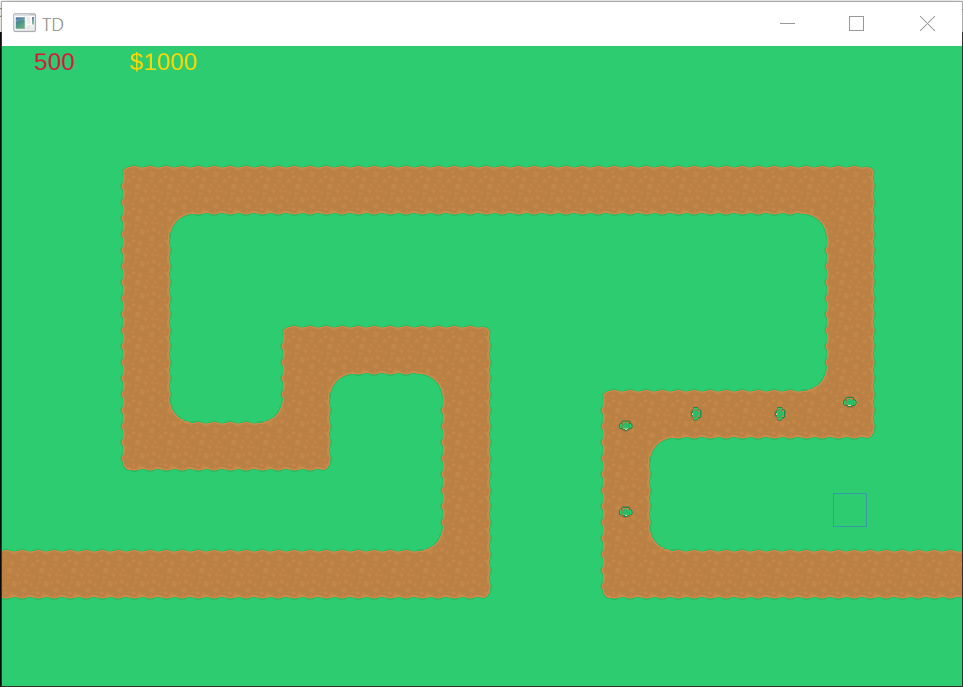
\includegraphics{images/hra.png}
    \caption{Mapa a používateľské rozhranie}
\end{figure}

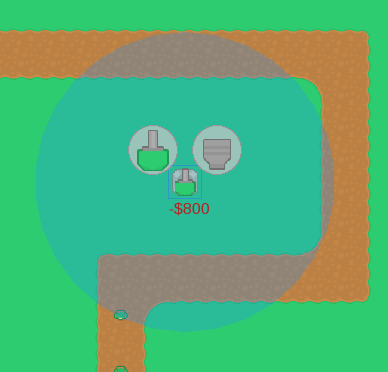
\includegraphics{images/contextmenu.png}

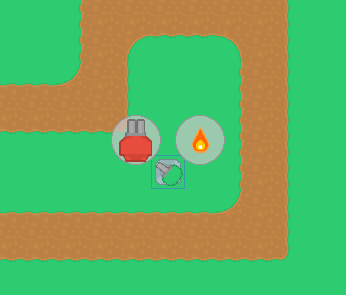
\includegraphics{images/upgrade.png}

\subsection{Protivníci}


\includegraphics{images/oponenti.png}


\includegraphics{images/lietadlo.png}

\subsection{Typy veží}


\includegraphics{images/veze.png}


\includegraphics{images/raketomet.png}

\section{Programátorská príručka}

\subsection{Vstupný bod a smyčka}
Hlavnú úlohu zohráva trieda \emph{App}. Jej metóda \emph{load} je zavolaná práve raz vo vstupnom
bode programu. Táto metóda sa postará o načítanie všetkých textúr, fontov a zvukov.
Následne metóda loop spustí hernú smyčku (game loop). Trieda \emph{App} pracuje so scénami.
Scéna je analógia jednej stránky vrámci webstránky. \emph{App} vlastní najviac jednu inštanciu
scény a rieši prechody medzi scénami, keď si to scéna vyžiada.

Game loop sa opakuje kým je okno aplikácie otvorené. Pozostáva z nasledujúcich častí:

\begin{enumerate}
    \item Prechod medzi scénami, ak si to práve aktívna scéna vyžiadala. \emph{App} predá
    konštruktoru novej scény parametre z objektu \emph{SceneChangeRequest}.
    \item Spracovanie vstupu - eventov. Napríklad kliky myšou, klávesnica apod.
    Pre každú udalosť - \emph{sf::Event} sa volá metóda \emph{Scene::handleInput(event)}.
    

    Toto je v aplikácií zaužívaný princíp. Objekty, ktoré vlastnia iné objekty,
    na nich volajú metódu \emph{handleInput(event)} pre každý obdržaný event.
    \item Niekoľko krokov v hernom svete \emph{fixedTimestepUpdate}, používa sa \emph{fixed timestep update},
    To znamená, že v každom cykle sa spraví toľko krokov v hernom svete, aby sa za každú sekundu spravilo 30 krokov.
    Scéna spraví krok po zavolaní \emph{update(delta)}. \emph{Delta} je časová dĺžka,
    o ktorý sa má svet pohnút dopredu. Keďže robím 30 krokov za sekundu, je to $\frac{1}{30}$ sekundy.
    
    
    Tento princíp sa zase opakuje naprieč celou aplikáciou. Rôzne objekty vo svojej metóde
    \emph{update} volajú \emph{update(delta)} na objekty, ktoré vlastnia.
    \item Kreslenie scény. Kresliteľné objekty dedia z triedy \emph{sf::Drawable} a implementujú
    jej virtuálnu metódu \emph{draw(target, states)} v ktorej vykreslia seba a objekty, ktoré vlastnia.
\end{enumerate}

\subsection{Scény}
Konkrétne scény sú implementované ako triedy, ktoré dedia zo \emph{Scene}. 
Scéna implementuje virtuálne metódy \emph{handleInput}, \emph{update} a \emph{draw} popísané
vyššie. Volaním metódy \\
\emph{requestSceneChange(request)} si scéna môže vyžiadať zmenu scény.


\emph{TextScene} je abstraktná scéna, ktorá vie zobraziť 3 texty a po stlačení niektorej
klávesy prejde do scény predanej konštruktoru.


Implementované sú nasledujúce scény:
\begin{itemize}
    \item \emph{WelcomeScene} je scéna so základnými informáciami, ktorá sa zobrazí
    po spustení aplikácie. Vychádza z \emph{TextScene}, po stlačení klávesy si vyžiada
    \emph{GameScen}, ktorej nepredáva žiadne informácie.
    \item \emph{GameScene} je samotná hra. Spravuje objekty užívateľského rozhrania
    \emph{ContextMenu} a \emph{StatusBar}, herný svet - \emph{World} a \emph{Director},
    ktorý riadi prichádzajúce vlny protivníkov. Zmena scény na \emph{GameOverScene} nastane
    v prípade, že zásahové body hráča klesnú na 0. Predáva sa posledné poradové
    číslo vlny pod parametrom \emph{waveNumber}.
    \item \emph{GameOverScene} informuje hráča o \emph{waveNumber}. Vychádza z \emph{TextScene}
    a po stlačení klávesy nastane prechod do \emph{GameScene}.
\end{itemize}


\subsection{Assets - textúry, fonty a audio}

Všetky obrázky sú od autora Kenney Vleugels. Nahrávajú sa ako jeden obrázok vo formáte png - \emph{tilesheet},
ktorý je rozdelený na štvorčeky veľkosti $64px\times64px$. Využíva sa jediný font Liberation Sans.
Zvukové efekty sú vytvorené v programe Bfxr.


Trieda Assets je singleton držiaci ukazovateľ na \emph{RenderWindow}, inštancie fontu, textúry a \emph{Audio}.
\emph{Audio} je dátová štruktúra, ktorá drží načítané zvuky a dokáže efektívne nájsť a prehrať poďla zadaného 
\emph{SoundEffect}. Singleton sa osvedčil ako lepšia možnosť oproti alternatívam, keďže takmer každý objekt potrebuje
mať prístup k aspoň jednej položke zo štvorice textúra, font, zvuk, okno.

\subsection{Sektor a mriežka}

Terén hry je rozdelený na štvorce veľkosti 64x64 bodov. Polohu tákehoto štvorca (sektoru) reprezentuje trieda
\emph{Sector}. Sektory majú vlastný súradnicový systém zložený z dvoch čísel. Sektor v ľavom hornom rohu má súradnice
$(0, 0)$, ktoré rastú smerom dole doprava. Niekedy je nutné prejsť od súradníc hry do súradníc sektoru alebo naopak.
Na to poskytuje \emph{Sector} metódy \emph{fromCoords}, \emph{upperLeftPoint} apod.


Mriežka \emph{(Grid)} je obdĺžnik zložený zo sektorov, ktoré majú priradenú textúru. Textúra priradená sektoru je 
reprezentovaná číslom štvorčeku vrámci tilesheetu. Je to rovnaké číslovanie ako využíva program Tiled, teda štvorčeky
v prvom riadku zhora sú očíslované zľava doprava 0, 1, ... 22, v druhom riadku 23, 24 ... apod. Toto číslo sa v zdrojových
kódoch označuje \emph{textureId}. Mriežka taktiež udržuje cestu - \emph{Path},
čo predstavuje lomenú čiaru vrámci mapy, po ktorej sa hýbu oponenti.


Vlna \emph{(Wave)} predstavuje jednu postupnosť protivníkov rovnakého typu so zadanými rozostupmi.
Na požiadanie ich dokáže vygenerovať - metóda \emph{maybeSendNext(delta)} buď vytvorí protivníka umiestniteľného do sveta
alebo vráti \emph{nullptr}. Robí to tak, aby boli dodržané dané časové rozostupy.


\emph{Director} vytvára a riadi vlny protivníkov. Vždy má najviac jednu inštanciu vlny, z ktorej posiela protivníkov do sveta.
Keď sa svet vyčistí (neobsahuje žiadneho protivníka), vytvorí si nasledujúcu vlnu. Prvých dvadsiatka vĺn je explictine definovaná,
ostatné sa generujú s lineárne sa zvyšujúcim počtom protivníkov.

\subsection{Herný svet - World}

\emph{World} je kontajner spájajúci mriežku, entity (veže, projektily, oponenti) a stav (koľko má hráč peňazí a zásahových bodov).


Entita \emph{Entity} je spoločný predok veží, projektilov a oponentov. Vlastní jeden \emph{(sf::Sprite)}, ktorému
priradí textúru podľa ID v konštruktore. Ponúka k nemu metódy, ktoré ho dokážu otočiť v smere vektoru alebo posunút so zadanou
rýchlosťou pohybu.


\emph{Actor} predstavuje jedneho oponenta. Je to entita pohybujúca sa po zadanej lomenej čiare. Udržuje si svoje zasáhové body, ktoré
mu uberajú projektily. Oponent skončí svoju púť keď prišiel o zásahové body alebo prešiel celú svoju dráhu. \emph{World} odchytáva tieto
situácie a príslušnemení svoje stavy. Buď navýši hráčove konto alebo zníži jeho zásahové body o hodnotu \emph{Actor::getWorth()} (respektíve).
Odvodené triedy \emph{Soldier} a \emph{Plane} sú konkrétne implementácie oponentov. Sú čisto dátové - len predávajú konkrétne hodnoty 
konštruktoru \emph{Actor}, ale návrh je pripravený tak, že by mohli obsahovať aj nejaké špecifické správanie.


\emph{Projectile} je projektil naháňajúci oponenta vo svete. Keď ho chytí, zníži mu zásahové body. V prípade, že oponent stihne zmiznúť
pred tým, ako ho projektil chytí, tak zmizne aj projektil. Projektily sú umiestňované do sveta vežami.
Implementovaný je \emph{Bullet} a \emph{Rocket}. Tieto sa líšia aj behaviorálne - raketa sa vzhľadom k svojej textúre otáča smerom k cieľu
a navyše akceleruje.


Veža \emph{Tower} môže byť hráčom umiestnená na akékoľvek políčko, kde neprechádza cesta. Potom prehľadáva pole oponentov
a keď je nejaký v dosahu, teda bližšie ako \emph{Tower::getRange()}, vystrelí naňho projektil. Vystreliť potom môže až keď
ubehne čas \emph{Tower::cooldown}. Implementácie veží sú \emph{GreenGun}, \emph{RedTwinGun} a \emph{RocketLauncher}. Líšia sa
číslami, ktoré predávajú konštruktoru \emph{Tower} a spôsobom vytvárania projektilov. \emph{RedTwinGun} vyrába projektily tak,
aby sa zdalo že vybiehajú striedavo z ľavej a pravej hlavne. \emph{RocketLauncher} zase striela rakety.
Všetky konkrétne veže obsahujú svoje vlastnosti ako verejné statické atribúty. Toto umožňuje použitie metaprogramovania v časti UI.

\section{Užívateľské rozhranie}

\emph{TowerPreview} je náhľad veže, ktorá ešte nie je umiestnená vo svete. Využíva sa pred kúpou alebo pred vylepšením veže.
Naznačuje kde bude veža umiestená, aký bude mať dostrel a koľko to bude stáť.


\emph{Button} je všeobecné tlačítko reagujúce na polohu myši a na kliknute. Rozpozná, keď je myš nad ním, a konkrétna implementácia
tlačítko sa ho na to môže spýtať volaním \emph{Button::mouseHovers}. Pri kliku zavolá virtuálnu metódu \emph{onClick}. Táto metóda by mala
byť zavolaná aj v každej implementácii tlačidla, aby si trieda \emph{Button} správne zaznačila, že tlačidlo už bolo zatlačené.


\emph{PlaceTowerButton<T>} je tlačítko umiesťnujúce vežu typu \emph{T}. Stará sa zobrazenie náhladu a pri kliku aj o odpočítanie ceny veže
a umiestnenie veže do sveta. \emph{UpgradeTowerButton<T>} zase dokáže "vylepšiť" vežu - prakticky zmazať starú vežu, umiestniť na rovnaké miesto
novú a odpočítať rozdiel v cenách. \emph{SellTowerButton} vežu odstráni a pripíše hráčovi na konto polovicu pôvodnej ceny.  


\emph{ContextMenu} zobrazuje pod myšou hráća indikátor, aby hráč videl nad ktorým sektorom sa nachádza.
Sú dva druhy kontextových menu - nad prázdnym políčkom, kde je možné postaviť vežu, sa zobrazí "shopping list"
teda ponuka dvoch tlačítok na kúpenie veže. Toto sú \emph{PlaceTowerButton<GreenGun>} a \emph{PlaceTowerButton<RocketLauncher>},
Nad políčkom, kde je umiestnená veža, máme možnosť predaja - tlačítko \emph{SellTowerButton}, prípadne \emph{UpgradeTowerButton<typVežeNaSektore>}.
Sektory cesty sú naznačené červeným indikátorom a nemajú žiadne kontextové menu.

\end{document}
